\documentclass[11pt]{article}
\usepackage[utf8]{inputenc}
\usepackage[spanish,es-tabla]{babel}
\usepackage{amsmath}
\usepackage{amsfonts}
\usepackage{amssymb}
\usepackage{graphicx}


\usepackage{hyperref}
\usepackage{float}
\usepackage[a4paper,top=1.5cm,bottom=0cm,left=1.5cm,right=1.5cm,marginparwidth=1.75cm]{geometry}


\title{Tubbing S.A \\ \small{Comunicaciones digitales} \\ \small{Universidad Nacional del Comahue} }
\author{ 
        Gatica, Isaias \\ \small{LautaroAndresSaez@gmail.com} \and 
        Millain, Gonzalo \\ \small{gonza.pm@outlook.com} \and
        Saez, Lautaro Andres \\ \small{IsaiasGatica1@gmail.com} 

}
\date{}

\begin{document}
    \maketitle
    \section{Generalidades}
    
        \subsection{Estructuras de redes}
        \begin{figure}[H]
            \centering
            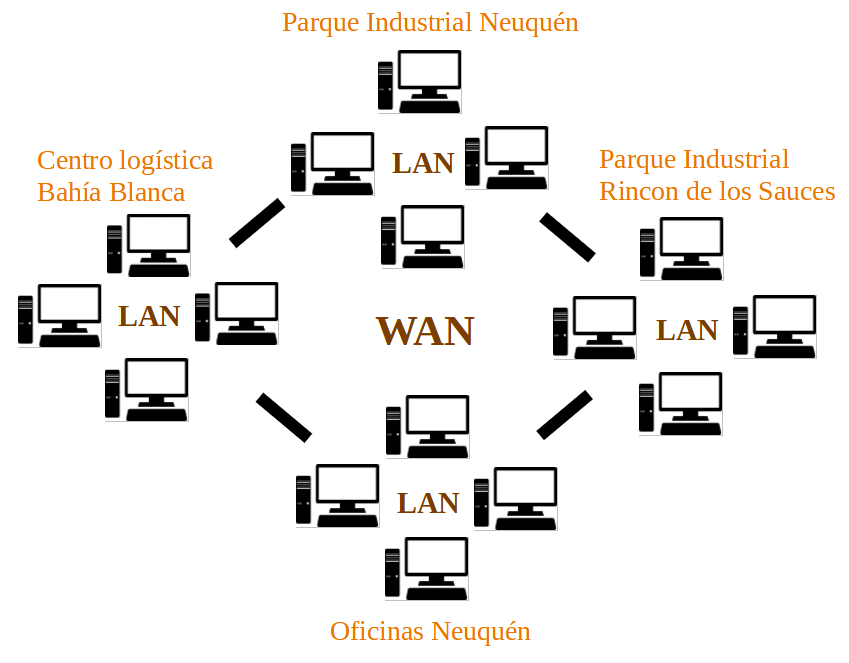
\includegraphics[scale=0.5]{Figure/Tubbin_Estructura.PNG}
            \caption{Imagen representativa de la estructura de Red}
            \label{Estructura}
        \end{figure}


        \subsubsection*{LAN}

        Cada area tendra su propia red LAN, la cual mas adelante se definira si sera por cable o WiFi dependiendo de las 
        prestaciones necesarias para cada lugar. Como primer medida adoptaremos el protocolo Ethernet por ser el mas utilizado.

        \subsubsection*{WAN}

        Se tendra una red WAN que realize una interconexión entre todas las areas con la central que estara ubicada en Parque Industrial.
        Esto permitira mediante una red Proxy/VPN facilitando el teletrabajo.

        \subsubsection*{Seguridad}

        Para aumnetar la seguridad de la red WAN/LAN y tener un mayor control del uso de la red y quienes usan dicha red 
        se decide implementar un servidor Proxy y/o un VPN.

        \subsection{Servicios de terceros}

        Debido a la complejidad de montar algunos sistemas y costo que esto conlleva se decidio tomar servicios de terceros, los 
        cuales se nombran a continuación.

        \subsubsection*{Servidor remoto}

        Con la finalidad de disminuir el costo de mantenimiento de un servidor y los cambios en la infraestructura que esto llevaria se 
        alquilara un servidor. Los precios de estos servidores rondan entre los $\$5000$ y $\$20000$ por mes, en este 
        caso nos decantariamos por un servicio intermedio el cual cuesta $\$6000$. El provedor es \href{https://www.hostdime.com.ar/servidores-dedicados}{hostdime}.

        \subsubsection*{Flota de camiones}

        Dada la importacia de realizar un seguimiento de la flota de camiones y el bajo costo de alquilar un servicio.
        Tomando como referencia $\$800$ por camion del servicio \href{https://galileosatelital.com/rastreo-vehicular-gps}{Galileo}.
        
    \section{Diseño de redes LAN}

    \subsection*{Parque Central}

        Los Switch a utilizar serán $2$ \href{https://articulo.mercadolibre.com.ar/MLA-714545399-switch-cisco-semi-admin-24-puertos-10100-2-giga-sf220-24-k9-_JM#position=34&type=item&tracking_id=4df4b6b4-1084-45cf-bab2-a07d312cf877}{Stiwch Cisco SF220-24-K9}
        cuyo precio ronda lo $\$18000$.


        Se deciden armar las siguienres VLAN's: 

        \begin{enumerate}
            \item Camaras de seguridad: ... 
            \item Gerencia y reuniones y oficinas: ...  
            \item Laboratorio: ...
            \item Refrigerios y limpieza: El cual lleva una red WiFi sin VPN para que los empleados puedan entrar a redes sociales, y 
                consumir contenido multimedia.
            \item Planta industrial: Para lograr una intercoxion entre los PLC's.
        \end{enumerate}

        \textbf{CONSULTAR TEMA ROUTER !!!}
        

    \subsection*{Parque industrial Rincón de los Sauces}

    Se utiliza un switch Cisco SF220-24-K9. Y se implementaran las siguientes VLAN's: 

    \begin{enumerate}
        \item Camaras de seguridad: 
        \item Oficinas 
        \item Intrumentos: 
        \item Refrigerio, limpieza y sanitarios: Red WiFi sin VPN. 
    \end{enumerate}

    \subsection*{Oficinas comerciales Neuquén}

    Ver swich o router

    \subsection*{Centro de logística Bahía Blanca}

    Ver switch o router  

    \end{document}
